% Restore modern floats after loading the original institutional class.
\makeatletter\let\KavachOriginalFloat\@xfloat\makeatother
\documentclass[a4paper,12pt]{nitathesis}
\makeatletter\let\@xfloat\KavachOriginalFloat\makeatother
\usepackage[T1]{fontenc}
\usepackage[utf8]{inputenc}
\usepackage{graphicx,times,amsmath,amssymb}
\usepackage[Sonny]{fncychap}
\usepackage{booktabs,tabularx,longtable,array}
\usepackage{tikz}
\usetikzlibrary{arrows.meta,positioning}
\usepackage{listings}
\usepackage[hidelinks,breaklinks,hypertexnames=false]{hyperref}
\usepackage{etoolbox}
% Report details confirmed by the candidate in PDF review comments.
\newcommand{\ReportTitle}{KAVACH: User Login Analysis Using LLM}
\newcommand{\CandidateName}{Umakant Yadav}
\newcommand{\RollNumber}{24MCA026}
\newcommand{\DegreeName}{Master of Computer Applications}
\newcommand{\DegreeShort}{MCA}
\newcommand{\SupervisorName}{Dr. Ranjita Das}
\newcommand{\SupervisorDesignation}{Assistant Professor}
\newcommand{\HodName}{Dr. Ashim Saha}
\newcommand{\HodDesignation}{Associate Professor}
\newcommand{\SubmissionDate}{November, 2026}

\hypersetup{pdftitle={\ReportTitle},pdfauthor={\CandidateName},pdfsubject={MCA project report}}
\makeatletter
\patchcmd{\@makechapterhead}{\vspace*{50\p@}}{\vspace*{0\p@}}{}{}
\patchcmd{\@makeschapterhead}{\vspace*{50\p@}}{\vspace*{0\p@}}{}{}
\makeatother
\setlength{\headheight}{15pt}
\setlength{\parskip}{7pt}
\setlength{\emergencystretch}{3em}
\widowpenalty=10000\clubpenalty=10000
\numberwithin{figure}{chapter}
\renewcommand{\headrulewidth}{0.5pt}
\renewcommand{\footrulewidth}{0.5pt}
\fancyhf{}\fancyhead[RO,LE]{\small\nouppercase{\leftmark}}\fancyfoot[C]{\thepage}
\renewcommand{\chaptermark}[1]{\markboth{\thechapter. #1}{}}
\newcolumntype{Y}{>{\raggedright\arraybackslash}X}
\lstset{basicstyle=\ttfamily\footnotesize,breaklines=true,columns=fullflexible,keepspaces=true,frame=single,showstringspaces=false}
\definecolor{KBlue}{HTML}{164E87}
\definecolor{KTeal}{HTML}{087F8C}
\definecolor{KPurple}{HTML}{7041A5}
\definecolor{KAmber}{HTML}{9A6500}
\definecolor{KRed}{HTML}{B33D59}
\definecolor{KGray}{HTML}{526174}
\tikzset{box/.style={draw=KBlue,fill=KBlue!7,rounded corners=2pt,align=center,text width=4.2cm,minimum height=1.1cm,font=\small},flow/.style={-{Latex[length=2.5mm]},thick,draw=KBlue}}
% Editable vector diagram styles. No raster artwork is used.
\tikzset{
 dbase/.style={draw,line width=.7pt,rounded corners=2pt,align=center,inner sep=7pt,minimum height=1.05cm,font=\small},
 person/.style={dbase,draw=KGray,fill=KGray!9},
 app/.style={dbase,draw=KBlue,fill=KBlue!9},
 store/.style={dbase,draw=KTeal,fill=KTeal!9,rounded corners=0pt},
 ai/.style={dbase,draw=KPurple,fill=KPurple!9},
 check/.style={dbase,draw=KAmber,fill=KAmber!10},
 alert/.style={dbase,draw=KRed,fill=KRed!8},
 note/.style={dbase,draw=KGray!65,fill=KGray!4,font=\footnotesize},
 dep/.style={-{Latex[length=2.1mm]},draw=KBlue,line width=.8pt},
 ret/.style={dep,dashed},
 assoc/.style={draw=KGray,line width=.7pt},
 edge/.style={font=\scriptsize,align=center,fill=white,inner sep=2pt,text=black},
 boundary/.style={draw=KGray!70,dashed,rounded corners=3pt,line width=.7pt}
}
\newcommand{\dn}[6]{\node[#1,text width=#5cm] (#2) at (#3,#4) {#6};}
\newcommand{\legendline}{\par\noindent{\footnotesize\textcolor{KBlue}{Blue: application}\quad\textcolor{KTeal}{Teal: data}\quad\textcolor{KPurple}{Purple: AI}\quad\textcolor{KAmber}{Amber: decisions}\quad\textcolor{KGray}{Gray: actors / boundaries}}\par}
\newcommand{\actor}[4]{%
 \begin{scope}[shift={(#2,#3)},draw=KGray,line width=.9pt]
 \draw[fill=KGray!8] (0,.43) circle (.18);
 \draw (0,.25)--(0,-.28) (-.3,.03)--(.3,.03) (0,-.28)--(-.27,-.63) (0,-.28)--(.27,-.63);
 \coordinate (#1) at (0,0);
 \node[font=\small,align=center,text width=2.5cm] at (0,1.1) {#4};
 \end{scope}}

\newcommand{\code}[1]{\nolinkurl{#1}}
\newcommand{\fronttitle}[1]{\clearpage\thispagestyle{plain}\begin{center}\LARGE\bfseries #1\end{center}\vspace{1.2cm}}
\newcommand{\facultyblock}[3]{\begin{minipage}[t]{0.46\textwidth}\centering\rule{6cm}{0.4pt}\\#1\\#2\\#3\\\small Computer Science and Engineering\\NIT Agartala\end{minipage}}
\begin{document}
\pagenumbering{roman}\pagestyle{plain}
\begin{titlepage}\centering
{\LARGE\bfseries\MakeUppercase{\ReportTitle}\par}
\vspace{2.2cm}
\includegraphics[width=4.4cm]{images/nita_logo.png}\par
\vspace{1.5cm}{\large\bfseries\DegreeName\ Project Report\par}
\vspace{0.8cm}{\large\bfseries\CandidateName\ (\RollNumber)\par}\vfill
{\bfseries COMPUTER SCIENCE \& ENGINEERING DEPARTMENT\\NATIONAL INSTITUTE OF TECHNOLOGY, AGARTALA\\INDIA--799046\par}
\vspace{0.6cm}{\bfseries\SubmissionDate\par}\end{titlepage}
\begin{titlepage}\centering
{\LARGE\bfseries\MakeUppercase{\ReportTitle}\par}\vspace{0.8cm}
{\bfseries\itshape Report submitted to\\National Institute of Technology, Agartala\\for the award of the degree of\\\large\DegreeName\par}\vspace{0.5cm}
{\bfseries\itshape by\\\CandidateName\ (\RollNumber)\par}\vspace{0.7cm}
{\bfseries\itshape Under the Guidance of\\\SupervisorName\\\SupervisorDesignation\par}
\vspace{0.7cm}
\includegraphics[width=4cm]{images/nita_logo.png}\par\vfill
{\bfseries COMPUTER SCIENCE \& ENGINEERING DEPARTMENT\\NATIONAL INSTITUTE OF TECHNOLOGY AGARTALA\par}
\vspace{0.4cm}{\bfseries\SubmissionDate\par}\end{titlepage}
\setcounter{page}{3}
\fronttitle{Dedicated To}
\begin{center}\begin{minipage}{0.86\textwidth}
To my project supervisor, \SupervisorName, \SupervisorDesignation, CSED, NIT Agartala, for guidance, insight, encouragement, and trust throughout this project. I also thank the faculty members of the department for their teaching and support in my professional growth. I dedicate this work to everyone who helped develop the project and supported me along the way.
\end{minipage}\end{center}
\fronttitle{REPORT APPROVAL FOR \DegreeShort}
This report entitled ``\ReportTitle'', submitted by \CandidateName\ (\RollNumber), is presented in partial fulfilment of the requirements for the award of the \textbf{\DegreeName} degree at the National Institute of Technology, Agartala.
\vspace{2.5cm}\par\noindent
\facultyblock{\SupervisorName}{(Project Supervisor)}{\SupervisorDesignation}\hfill\facultyblock{\HodName}{(Head of the Department)}{\HodDesignation}
\vspace{2cm}\par\noindent Date: \rule{5cm}{0.4pt}\\Place: NIT Agartala
\fronttitle{DECLARATION}
I declare that this report, ``\ReportTitle'', submitted to the Department of Computer Science and Engineering, National Institute of Technology, Agartala, for the \DegreeName\ degree, presents my work. I have acknowledged the sources used in preparing it. I understand my responsibility to uphold academic honesty and integrity, including the prohibition on fabricating results, data, or references.

The candidate must review and sign this declaration before submission.
\vspace{2cm}\par\hfill\begin{minipage}{7cm}\centering\rule{6cm}{0.4pt}\\\CandidateName\\\RollNumber\end{minipage}
\vspace{1.2cm}\par\noindent\SubmissionDate\\NIT Agartala
\fronttitle{CERTIFICATE}
The report titled ``\ReportTitle'', submitted by \CandidateName\ (\RollNumber), is presented for certification of the project work carried out under the guidance of the project supervisor towards the \DegreeName\ degree.

Certification and approval require review and signatures from the supervisor and the department.
\vspace{2.5cm}\par\noindent
\facultyblock{\SupervisorName}{(Project Supervisor)}{\SupervisorDesignation}\hfill\facultyblock{\HodName}{(Head of the Department)}{\HodDesignation}
\vspace{2cm}\par\noindent Date: \rule{5cm}{0.4pt}\\Place: NIT Agartala
\prefacesection{Acknowledgement}
I thank my project supervisor, \SupervisorName, \SupervisorDesignation, for guidance, feedback, and encouragement during the development of KAVACH. I am grateful to \HodName, \HodDesignation\ and Head of the Department, and to the faculty of the Department of Computer Science and Engineering, National Institute of Technology Agartala, for their academic support.

The developers and maintainers of Spring Boot, Spring Security, React, PostgreSQL, and the supporting open-source libraries made this project possible. Their software provided a foundation for studying authentication monitoring, rule-based anomaly detection, and security analysis with application tools. I also thank my family and friends for their patience and support.
\vspace{1cm}\par\hfill\CandidateName\ (\RollNumber)
\clearpage\begingroup\setlength{\parskip}{0pt}\setstretch{1.05}\listoffigures\endgroup\clearpage\begingroup\setlength{\parskip}{0pt}\setstretch{1.05}\listoftables\endgroup
\prefacesection{Abstract}
KAVACH monitors login activity and applies explicit rules to identify unusual events. It provides an AI tool interface for investigating those events. A React frontend communicates with a Java 21 Spring Boot backend, which stores data in PostgreSQL through Spring Data JPA. BCrypt verifies passwords, and bearer JSON Web Tokens authenticate later requests. Role and ownership checks protect administrative operations and selected account resources.

The detector checks six conditions: a failed login, a login at an unusual hour, an inactive account, an unseen IP address, an unseen device string, and repeated failures within a ten-minute window. Each matching rule assigns a fixed severity and weight. The user risk score sums anomaly weights from the preceding 24 hours and caps the result at 100. The dashboard presents login statistics, severity totals, recent critical anomalies, and a ranked account watchlist.

The AI service produces structured anomaly explanations and runs a two-loop workflow. The inner loop executes bounded model or planner cycles and application tools; the outer loop processes follow-ups supplied with the request. Thirteen registered tools provide investigative queries and selected account or telemetry operations. A deterministic fallback handles requests when live inference is unavailable. This report describes the implementation, data flows, detection rules, and a reproducible validation plan. Accuracy, throughput, and production readiness have not been measured; proposed improvements are identified separately from implemented behavior.

\noindent\textbf{Keywords:} authentication telemetry, anomaly detection, risk scoring, Spring Security, two-loop agent, security dashboard.
\clearpage\begingroup\setlength{\parskip}{0pt}\setstretch{1.05}\tableofcontents\endgroup
\clearpage\pagenumbering{arabic}\pagestyle{fancy}\raggedbottom
\chapter{Introduction}
\section{Project Overview}
Login records help investigators examine account misuse. Each record identifies an account, an outcome, a time, and network or client details. A single event provides limited context. Comparing it with account state and earlier activity can explain why it deserves attention.

KAVACH brings login records, rule-based alerts, account risk, audit history, and AI-assisted investigation into one web application. Its name means a shield. The application has a Spring Boot REST backend, a React frontend, and PostgreSQL storage. The implementation described here is the supplied source snapshot \cite{repo}.

ADMIN and USER are the application security roles. Administrators can inspect activity across accounts and manage users through designated endpoints. Ordinary users have selected views of their own activity. The AI investigator and operator roles describe agent behavior; they do not replace the signed-in user's permissions.

\section{Problem Statement}
Rejecting an incorrect password leaves an investigator to determine which account was targeted, whether failures repeated, and whether the client was familiar. KAVACH connects login records with alerts and recent account risk to support that investigation in a small application with inspectable logic.

The project evaluates login events with explicit rules, combines the resulting alerts into a bounded account score, and lets a conversational interface retrieve relevant application data through tools. Statistical validation and deployment hardening remain further work.

\section{Objectives}
\begin{enumerate}
\item Implement registration and authentication with encoded passwords and bearer tokens.
\item Persist login activity and evaluate six explicit detection rules.
\item Present anomalies, risk, trends, account status, and audit events through role-aware pages.
\item Support structured AI explanations with a deterministic fallback.
\item Implement bounded tool calling and continuation through supplied follow-ups.
\item Document the architecture and the tests needed to establish correctness and security.
\end{enumerate}

\section{System Block Diagram}
Figure~\ref{fig:architecture} shows the browser, API, service layer, and external dependencies. Browser requests go through the backend, which controls access to PostgreSQL and the model provider. Application services save records, evaluate rules, and coordinate AI requests.
\begin{figure}[htbp]\centering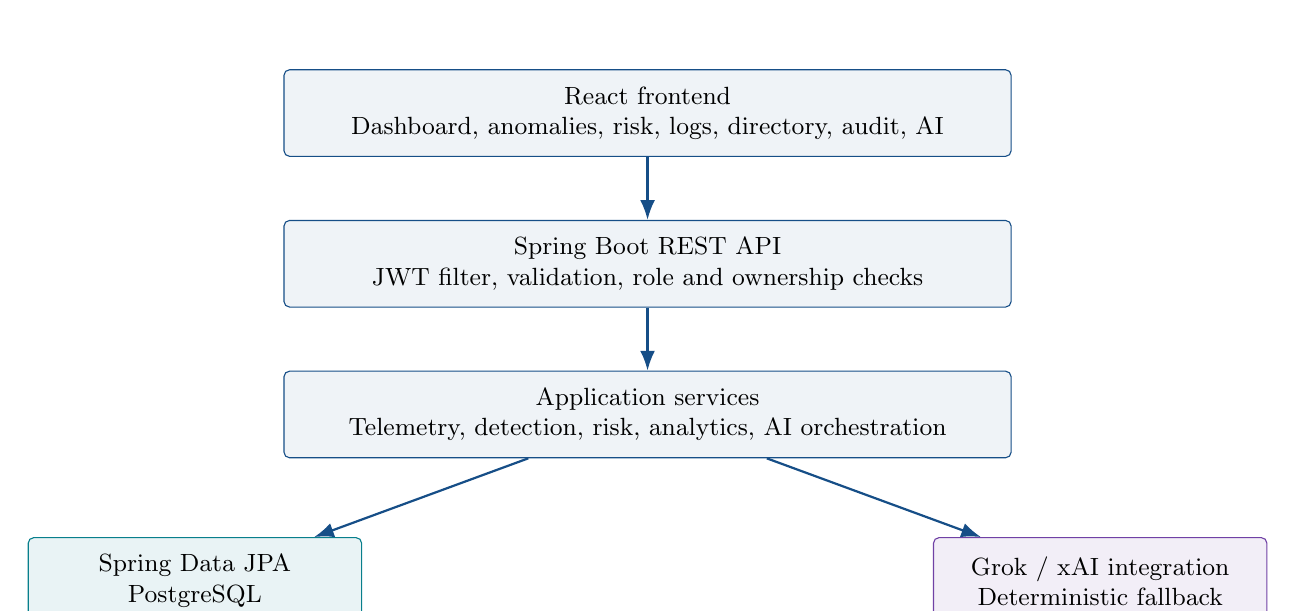
\begin{tikzpicture}[node distance=0.8cm]
\node[box,text width=9cm] (ui) {React frontend\\Dashboard, anomalies, risk, logs, directory, audit, AI};
\node[box,below=of ui,text width=9cm] (api) {Spring Boot REST API\\JWT filter, validation, role and ownership checks};
\node[box,below=of api,text width=9cm] (svc) {Application services\\Telemetry, detection, risk, analytics, AI orchestration};
\node[box,draw=KTeal,fill=KTeal!9,below left=1cm and -1cm of svc,text width=4cm] (db) {Spring Data JPA\\PostgreSQL};
\node[box,draw=KPurple,fill=KPurple!9,below right=1cm and -1cm of svc,text width=4cm] (ai) {Grok / xAI integration\\Deterministic fallback};
\draw[flow](ui)--(api);\draw[flow](api)--(svc);\draw[flow](svc)--(db);\draw[flow](svc)--(ai);
\end{tikzpicture}\caption{KAVACH implementation architecture.}\label{fig:architecture}\end{figure}

\section{Scope and Boundaries}
KAVACH is a prototype for monitoring activity within the application. Detection uses fixed rules without training a machine-learning model. The IP rule compares stored addresses and performs no external reputation lookup. The device rule compares supplied strings, including user-agent information captured during authentication; those strings do not verify a physical device.

The inactive-user rule reads the account active flag and does not measure how long an account has been dormant. Quarantine sets that flag to false, affecting later authentication and JWT checks. It provides no operating-system isolation or firewall enforcement.

The project materials contain no production traffic dataset, benchmark run, or labelled evaluation corpus. Detection accuracy and performance therefore remain unmeasured. Chapter 5 describes the interfaces and includes selected application screenshots supplied by the candidate.

\section{Organization of the Report}
Chapters 2--4 describe requirements, system design, and implementation. Chapter 5 presents the interfaces and validation plan. Chapter 6 discusses limitations and future work. The appendices contain the repository structure, database dictionary, API reference, publication statement, and biographical sketch.
\chapter{Requirement Analysis}
\section{Software Requirements}
The repository declares the dependencies in Table~\ref{tab:stack}. Development requires Java 21, a compatible Node.js environment, and PostgreSQL. Live inference also needs provider configuration and network access.
\begin{table}[!ht]\centering\footnotesize\setstretch{1.0}\renewcommand{\arraystretch}{1.1}\caption{Declared software stack.}\label{tab:stack}
\begin{tabularx}{\textwidth}{lY}\toprule Component & Declaration or purpose\\\midrule
Java & Version 21 in Maven properties.\\
Spring Boot & Parent 4.1.1; MVC, validation, JPA, and security starters.\\
PostgreSQL & JDBC driver and relational persistence.\\
JWT & JJWT API, implementation, and Jackson modules 0.12.6.\\
AI client & OpenAI Java SDK 4.101.0 for Grok integration.\\
React & React and React DOM \code{^19.3.1}.\\
Vite & Build dependency \code{^8.3.6}.\\
Presentation & Tailwind CSS \code{^3.4.17}, Recharts, Lucide React, GSAP.\\
HTTP / routing & Axios and React Router DOM.\\\bottomrule\end{tabularx}\end{table}

Maven wrapper scripts build the backend. The frontend has scripts for development, production builds, preview, and linting. Vite uses port 5173 and proxies \code{/api} to \code{http://localhost:8080}. The Axios client can also use a configured API base URL.

\clearpage\section{Functional Requirements}
\begin{enumerate}
\item Validate registration, reject duplicate usernames/emails, hash passwords, authenticate active accounts, and return JWTs with safe user details.
\item Record known-account login outcomes and permit administrator-created demonstration events with account, timestamp, status, IP, device, and location fields.
\item Evaluate six independent rules, preserve each triggered anomaly, and check the user/type/event combination before inserting a duplicate.
\item Aggregate recent anomalies into a capped 24-hour risk score and expose severity totals, login outcomes, a seven-day trend, and a ten-account watchlist.
\item Provide role-aware account, telemetry, anomaly, audit, and AI views; apply ownership checks to selected personal resources.
\item Support advisory explanations, analysis history, bounded tool calling, and deterministic fallback when live inference is unavailable.
\end{enumerate}

\section{Quality and Operating Requirements}
Protected requests must authenticate the caller and enforce role or ownership checks at sensitive entry points. Tool execution needs the same action-level policy. Alerts must preserve the matching rule, its reason, and its fixed weight. Controllers, services, repositories, DTOs, and pages divide these responsibilities across the application.

Reliability testing must check failed-login transactions, repeated detection, and recording failures. Performance testing must cover history queries, pagination, and AI requests with several execution cycles. UI screenshots provide no measure of load capacity or detection accuracy.

Report examples omit local configuration values. Timestamp rules use \code{LocalDateTime}, so deployment needs a consistent time convention. Demonstration events must be identifiable alongside real login evidence. The project has no established minimum hardware specification or calibrated attack probabilities.
\chapter{Design Analysis}
\section{Layered Design and Access Boundaries}
HTTP controllers validate inputs and pass work to services. Services apply business rules and use JPA repositories to read entities and calculate aggregates. DTOs define the API data contracts. React pages share authentication and theme state and send requests through an Axios client \cite{repo}.

Authentication routes are public; other requests pass through the security chain. The JWT filter validates the token, looks up the current account, rejects inactive users, and sets the account role. Method security and selected ownership checks then restrict access to resources \cite{spring}. Registry tools enter services through a separate path, which needs equivalent authorization.

The client sends JSON with bearer credentials and uses a 30-second timeout. Unauthorized responses clear stored session state. Agent execution can span several model and tool cycles, so its timeout, cancellation, and retry behavior need coordination with the client. Appendix C lists the direct endpoint scopes.

% Each detailed diagram retains its dedicated vector page.
\newsavebox{\KDiagramRaw}
\newsavebox{\KDiagramScaled}
\newcommand{\diagramview}[4]{%
\clearpage\section{#1}
#2
\legendline
\begin{figure}[!ht]\centering
\sbox{\KDiagramRaw}{\input{diagrams/#3}}
\ifdim\wd\KDiagramRaw>\textwidth
 \sbox{\KDiagramScaled}{\resizebox{\textwidth}{!}{\usebox{\KDiagramRaw}}}
\else\sbox{\KDiagramScaled}{\usebox{\KDiagramRaw}}\fi
\ifdim\dimexpr\ht\KDiagramScaled+\dp\KDiagramScaled\relax>16cm
 \resizebox*{!}{16cm}{\usebox{\KDiagramScaled}}
\else\usebox{\KDiagramScaled}\fi
\caption{#4}\end{figure}}

\diagramview{C4 Level 1: System Context}{Account users and administrators access the same KAVACH system with different permissions. The context view groups the frontend, backend, and database inside that boundary. The optional model provider is an external dependency.}{c4-context}{C4 system context: actors, KAVACH, and optional model provider.}

\diagramview{C4 Level 2: Containers}{KAVACH has three C4 containers: the React browser application, the Spring Boot backend, and PostgreSQL. A container here is an independently running application or data store; the repository does not establish a Docker deployment. The localhost proxy follows the Vite configuration.}{c4-containers}{C4 containers: browser application, backend application, database, and provider.}

\diagramview{C4 Level 3: Backend Components}{The backend contains security filters, controllers, domain and AI services, and repositories. Arrows show dependencies, so individual requests need only the relevant branches. Registry tools enter services outside controller methods and need their own authorization checks.}{c4-components}{C4 backend components and external dependencies.}

\diagramview{UML Component Architecture}{The browser and JVM are the execution environments in this component view. Dashed arrows show usage dependencies and required interfaces. Domain services handle identity, monitoring, risk, and audit. AI components provide advisory analysis, orchestration, and operational tools.}{uml-architecture}{UML component architecture with execution boundaries and required interfaces.}

\diagramview{UML Sequence: Authentication and Detection}{Authentication proceeds down the lifelines through calls (solid arrows) and responses (dashed arrows). For known accounts, the service attempts telemetry for successful, incorrect-password, and inactive-account outcomes. Unknown usernames produce an audit failure without a user-linked event. A recorded event can trigger several anomalies.}{sequence-login}{UML login sequence: credentials, audit, telemetry, rules, and response.}

\diagramview{UML Sequence: Two-Loop Investigation}{The outer loop handles the initial task and supplied follow-ups. Each inner invocation allows up to six model or planner cycles. Tools run in sequence and feed results back into the conversation. The registry accesses application services and repositories, with live inference as an optional dependency.}{sequence-agent}{UML agent sequence: request-local queues, bounded planning, tools, and trace.}

\diagramview{Entity-Relationship Diagram}{Users can have zero or more login records and anomalies. Each anomaly requires one user and one login event. AI history has optional links to either entity. The diagram includes mapped fields, keys, and multiplicities; cached identifiers and audit usernames have no declared foreign-key relationships.}{entity}{Detailed entity model with keys, fields, optional links, and multiplicities.}

\diagramview{UML Use-Case Diagram}{An administrator inherits ordinary authenticated use cases and has additional global and account-management operations. The external model service supports AI use cases. These associations describe intended application scope; equivalent restrictions still need enforcement in every agent tool.}{use-cases}{UML use cases: personal investigation, administration, and optional AI support.}

\diagramview{DFD Level 0: Context}{Requests and responses cross the boundary between one KAVACH process and three external entities: the account user, administrator, and optional model provider. Internal database stores first appear in the level 1 decomposition.}{dfd0}{DFD level 0: balanced context inputs and outputs.}

\diagramview{DFD Level 1: Processes and Stores}{Six processes handle identity and accounts, telemetry, detection, risk and analytics, AI investigation, and audit review. D1--D5 identify the five entity groups. Repeated actor and store symbols are aliases for the same entities. Risk is calculated on query; a detection write does not automatically run the risk process.}{dfd1}{DFD level 1: six logical processes, five data-store groups, and external flows.}

\diagramview{DFD Level 2: Anomaly Detection}{Process 3.0 dispatches the event to six independent rules, then checks duplicates before saving each matching anomaly. Solid arrows carry events or candidates; dashed arrows carry history and existence-query feedback. The first event establishes the IP/device baseline. The failure-count query has no explicit upper event-time bound.}{dfd2-detection}{DFD level 2 of process 3.0: six rules, historical reads, and anomaly persistence.}

\diagramview{DFD Level 2: AI Investigation}{Process 5.0 routes requests to dedicated advisory analysis or agent execution. The dedicated path explicitly saves structured history. The agent returns an execution trace and can query or change application data through tools. Each invocation needs checks for account scope and action permissions.}{dfd2-ai}{DFD level 2 of process 5.0: advisory analysis, model/planner, tools, and outputs.}


\chapter{Functioning of the System}
\section{Registration and Authentication}
Registration trims the username, normalizes email, checks duplicates, and encodes the password. It creates an active USER account, saves an audit event, and returns safe fields. Login checks passwords with BCrypt, a one-way hashing scheme.

An unknown username produces an audit failure and an unauthorized response, with no user-linked login record. A known inactive account is blocked, and the service attempts to record a failed login. It also records failed telemetry for an active account with an incorrect password. Valid credentials produce a JWT, a success audit entry, and successful login telemetry.

JWT represents claims in the format defined by RFC 7519 \cite{jwt}. The browser attaches the token to later requests. The backend validates it and rechecks the current account state. Browser logout clears local authentication data; it does not revoke the token on the server.

\section{Telemetry Recording}
The recording method has a \code{REQUIRES_NEW} annotation to preserve telemetry independently of a failed authentication transaction. It supplies missing IP, device, and location values, saves the event, and invokes detection. The caller catches recording exceptions, allowing the main login response to proceed if recording fails.

Administrators can create demonstration events with a user ID, timestamp, IP address, device, location, and status. Rules that use event time read the supplied login timestamp, including a historical one. Any resulting anomaly receives a separate timestamp when it is detected.

\section{Detection Engine}
\begin{table}[htbp]\centering\small\caption{Detection conditions and fixed weights.}\label{tab:rules}
\begin{tabularx}{\textwidth}{lYrr}\toprule Rule & Trigger & Weight & Severity\\\midrule
Failed login & Status is FAILED. & 20 & LOW\\
Unusual time & Login hour is at least 0 and less than 5. & 25 & LOW\\
Inactive user & Account active flag is false. & 80 & CRITICAL\\
New IP & More than one event and no other event has the same non-null IP. & 40 & MEDIUM\\
New device & More than one event and no other event has the same device, ignoring case. & 30 & MEDIUM\\
Brute force & Failed event with at least five failures after ten minutes before its timestamp. & 70 & HIGH\\\bottomrule\end{tabularx}\end{table}

The detector evaluates all six rules sequentially. A failed login at an unusual hour can produce two anomalies, plus another if it meets the brute-force threshold. Weights are constants without dataset-based probability calibration.

\subsection{Historical Baselines}
The IP and device rules search the account's stored history, excluding the current event by ID. Both require more than one event, so the first establishes a baseline without triggering either alert. Comparisons use all stored history, including failed events. Device matching ignores case.

The inactive-account rule reads a Boolean flag; it does not calculate dormancy from the last successful login. The IP rule supplies neither geolocation nor reputation information. Device strings identify reported client values without authenticating hardware.

\subsection{Time Windows and Duplicates}
For a failed event at $t_e$, the repository counts failures with $t_{login}>t_e-10\text{ minutes}$. The query has no upper bound $t_{login}\leq t_e$. With chronological live events, this approximates a recent ten-minute count. For a backdated event, later records can also enter the count.

Before saving, the detector checks for the same user ID, anomaly type, and login-event ID to prevent duplicates during sequential reanalysis. Concurrent requests could both pass this check. A unique constraint or locking policy needs verification under concurrent execution.

\section{Risk Calculation}
Let $A_u(t)$ be the anomalies detected for user $u$ after $t-24$ hours, with stored weight $w_a$. The user risk score is
\begin{equation}R_u(t)=\min\left(100,\sum_{a\in A_u(t)}w_a\right).\end{equation}
Scores below 30 are LOW, 30--59 are MEDIUM, 60--79 are HIGH, and 80 or above are CRITICAL. The risky-user count includes accounts whose recent sum is at least 60. The watchlist query groups anomalies by account, caps each score at 100, sorts in descending order, and returns up to ten accounts.

If a failed login also has an unseen IP address and device, the three matching rules contribute $20+40+30=90$, placing the account in the CRITICAL tier. This calculation illustrates the scoring logic and is not an observed attack result. Even the maximum score of 100 does not mean a 100 percent probability of compromise.

\section{Dashboard Composition}
The dashboard presents risk, login analytics, a watchlist, and recent critical anomalies. Some counts cover all stored records, account risk covers 24 hours, and the trend covers seven days. These periods matter when comparing figures. Global counts and watchlist accounts lead into detailed investigation.

\section{Two-Loop AI Orchestration}
An agent request contains a prompt and may include context, a role, steering messages, and follow-ups. The service creates a local conversation, execution-step lists, and queues populated from the request. The outer loop starts an inner invocation and then processes the supplied follow-ups.


At the start of each inner iteration, the service adds at most one queued steering message to the conversation. The model or fallback planner returns text and any tool calls. The service resolves each tool by name, executes it, and adds its result or error to the conversation for the next cycle. The inner loop can finish when no tool calls or steering remain, and each invocation has a six-iteration limit.

Each follow-up starts another inner invocation. The final response contains text, execution steps, tool names, loop counts, mode, model, and completion time. Investigator and operator specializations affect behavior within one service and conversation; they do not run as separate agents.

Steering and follow-ups are fixed when the request begins. This execution path has no channel for messages typed while it is running, so live steering requires further work. Tools run sequentially, including those whose metadata declares parallel safety.

\section{Security Tools Registry}
\begingroup\small\setstretch{1.1}\setlength{\parskip}{0pt}
\begin{longtable}{>{\raggedright\arraybackslash}p{7cm}>{\raggedright\arraybackslash}p{7.3cm}}
\caption{Thirteen registered tools.}\label{tab:tools}\\\toprule Tool & Purpose\\\midrule\endfirsthead
\toprule Tool & Purpose\\\midrule\endhead
\code{get_dashboard_security_metrics} & Combined dashboard metrics.\\
\code{list_anomalies} & Recent anomalies, optional severity and limit.\\
\code{get_anomaly_details} & Anomaly and linked login metadata.\\
\code{explain_anomaly} & Structured AI explanation.\\
\code{get_user_risk_profile} & Account's recent risk.\\
\code{get_top_risky_users} & Ranked watchlist.\\
\code{query_login_telemetry} & Login records and outcomes.\\
\code{simulate_login_event} & Insert an event and invoke detection.\\
\code{get_user_directory} & Directory information.\\
\code{update_user_account_status} & Activate or deactivate an account.\\
\code{create_directory_user} & Provision an account.\\
\code{query_audit_trail} & Audit records with optional filters.\\
\code{generate_security_summary} & AI-assisted security summary.\\\bottomrule
\end{longtable}
\endgroup

Each tool declares an argument schema, role, and safety metadata. Execution still needs argument validation and authorization for the caller, action, and resource. Permissions for operational tools must cover state changes as well as reads.

\section{Explanations, Fallback, and Audit}
Dedicated anomaly analysis checks resource access before requesting structured JSON with a summary, explanation, indicators, implications, recommendations, and confidence. If the provider or parser fails, it produces a deterministic advisory response. Analysis history saves the result and an advisory flag.

Operational tools can change account status and save audit events; their authorization needs separate assessment from advisory recommendations. OWASP logging guidance provides criteria for event selection, protection, and verification \cite{owasp}. The existing database logs have no demonstrated tamper evidence.
\chapter{Interfaces and Validation}
\section{Interface Overview}
Signed-in users can open the anomaly, risk, login-log, and AI investigation pages. Administrators also have navigation to the global dashboard, directory, and audit records. The backend decides whether a request is authorized, regardless of which links the frontend displays.

Login and registration sit outside the protected layout. The authentication context keeps the token and safe user details in local storage. The shared HTTP client attaches the bearer token and clears the session on relevant unauthorized responses. Directory controls change account state. The audit view displays security records, while the browser console provides diagnostics.

Users can filter anomalies by rule type and severity and inspect their event context. The risk page summarizes the preceding 24 hours. Login views show the records behind the alerts, including administrator-created demonstration events. In the AI workspace, users select investigator, operator, or collaborative behavior and submit a prompt with optional context, steering, and follow-up arrays. The returned trace shows tool outcomes.

\clearpage\section{Application Screenshots}
These six candidate-provided captures show sign-in, overall monitoring, event investigation, personal risk, and the AI workspace. Their displayed content is unchanged. Counts and scores belong to the captured demonstration state; they are not evaluation measurements.

\begin{figure}[!ht]\centering
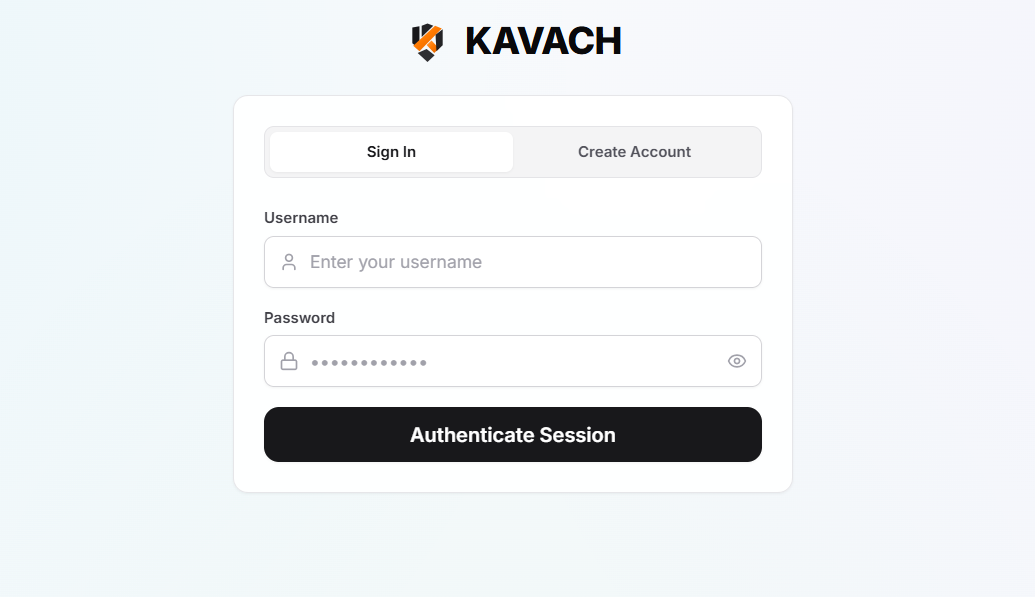
\includegraphics[width=.75\textwidth]{images/screenshot-login.png}
\caption{Sign-in interface with account-registration tab and authentication form.}\label{fig:screen-login}
\end{figure}

\begin{figure}[!ht]\centering
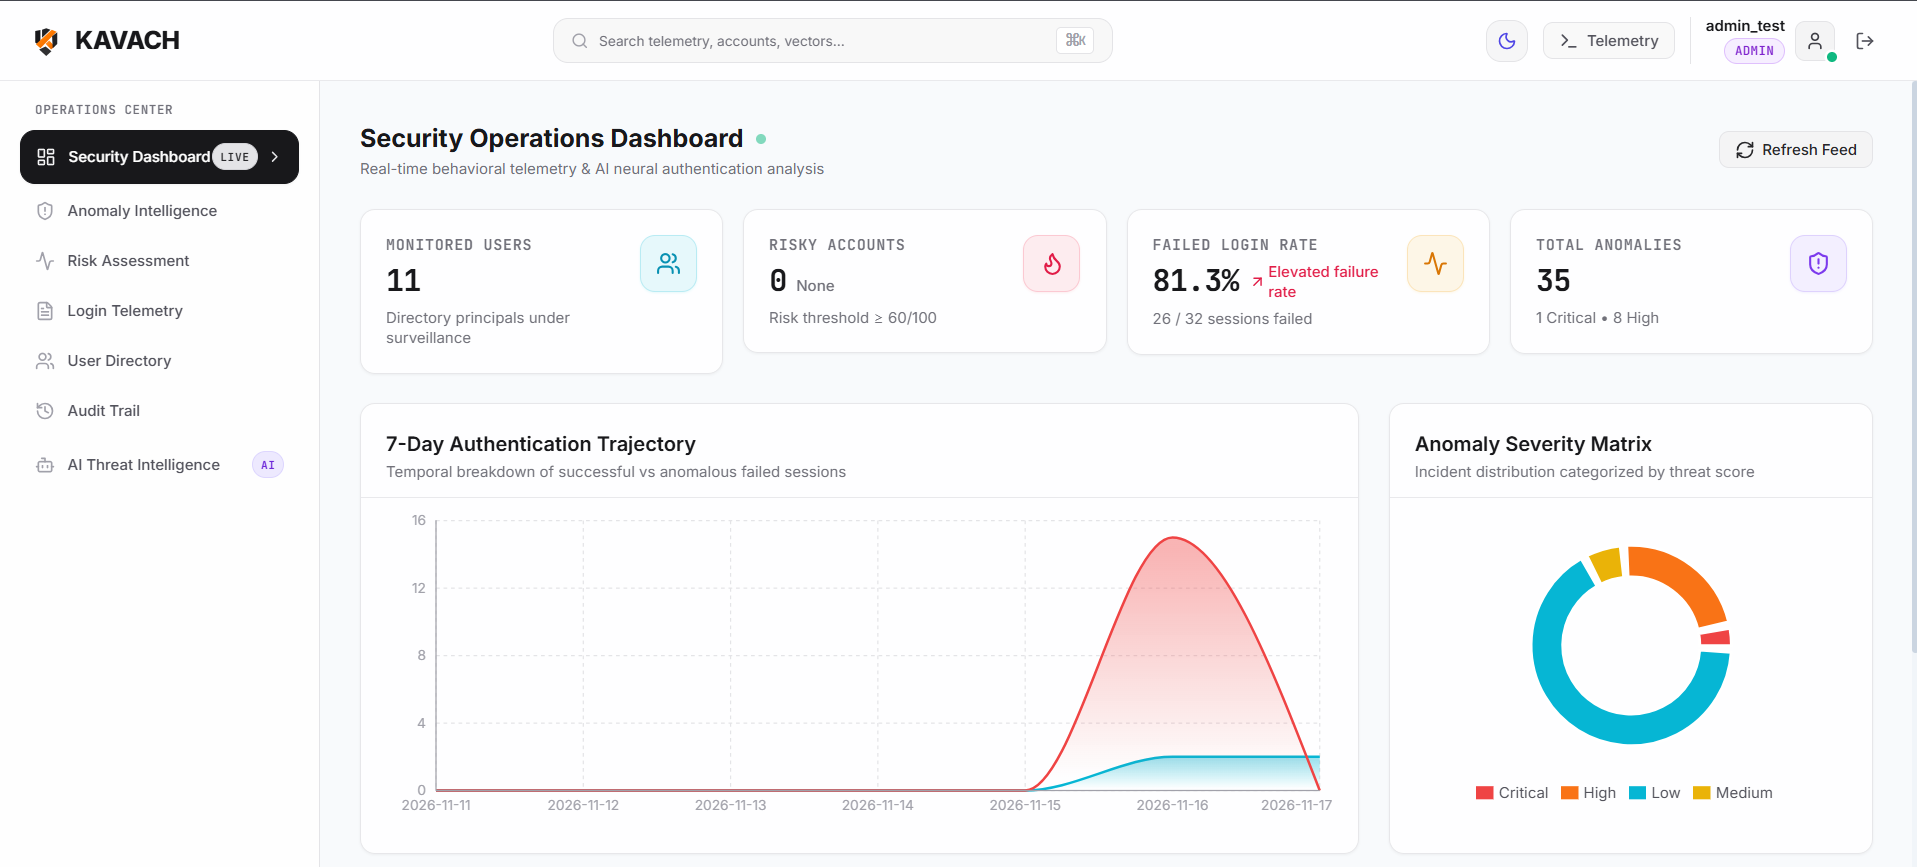
\includegraphics[width=\textwidth]{images/screenshot-dashboard.png}
\caption{Administrator dashboard: account counts, login outcomes, trend, and anomaly severity.}\label{fig:screen-dashboard}
\end{figure}

\clearpage\subsection{Anomaly Investigation and Login Telemetry}
The anomaly list shows matching rules and their alert weights. The login view provides the underlying event fields. Filters and action buttons are visible, but the captures do not show what happened after those actions were selected.

\begin{figure}[!ht]\centering
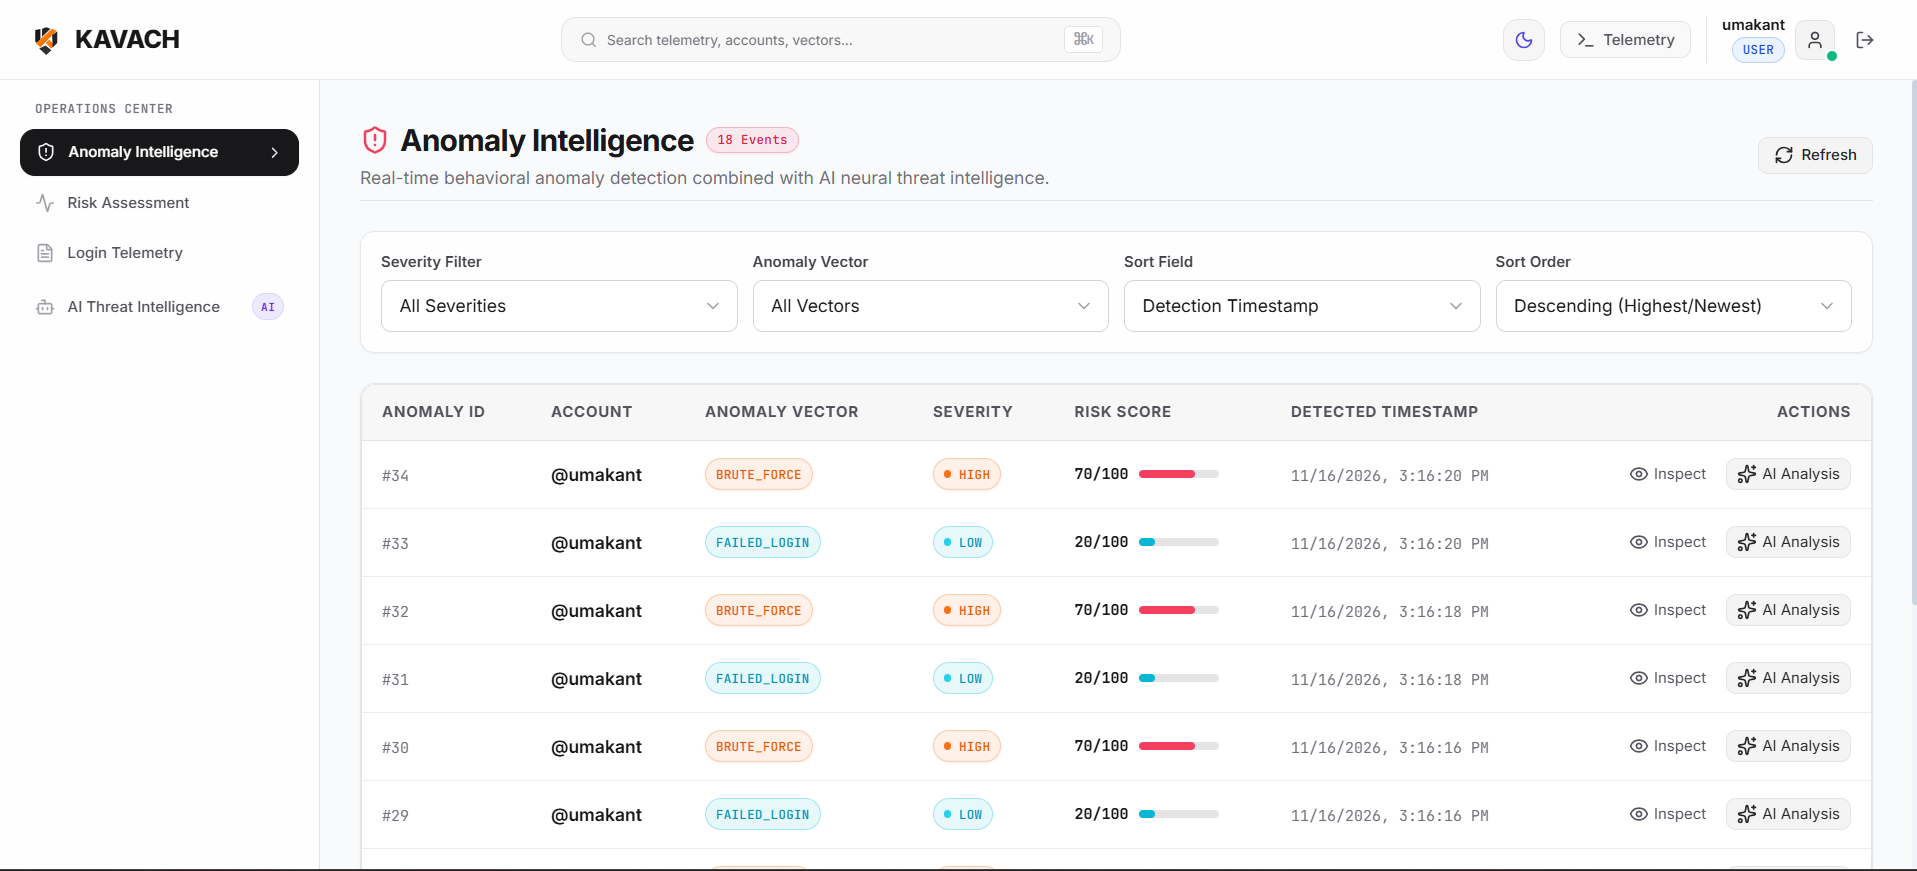
\includegraphics[width=\textwidth]{images/screenshot-anomalies.png}
\caption{User-scoped anomaly list with filters, rule types, severity, and alert weights.}\label{fig:screen-anomalies}
\end{figure}

\begin{figure}[!ht]\centering
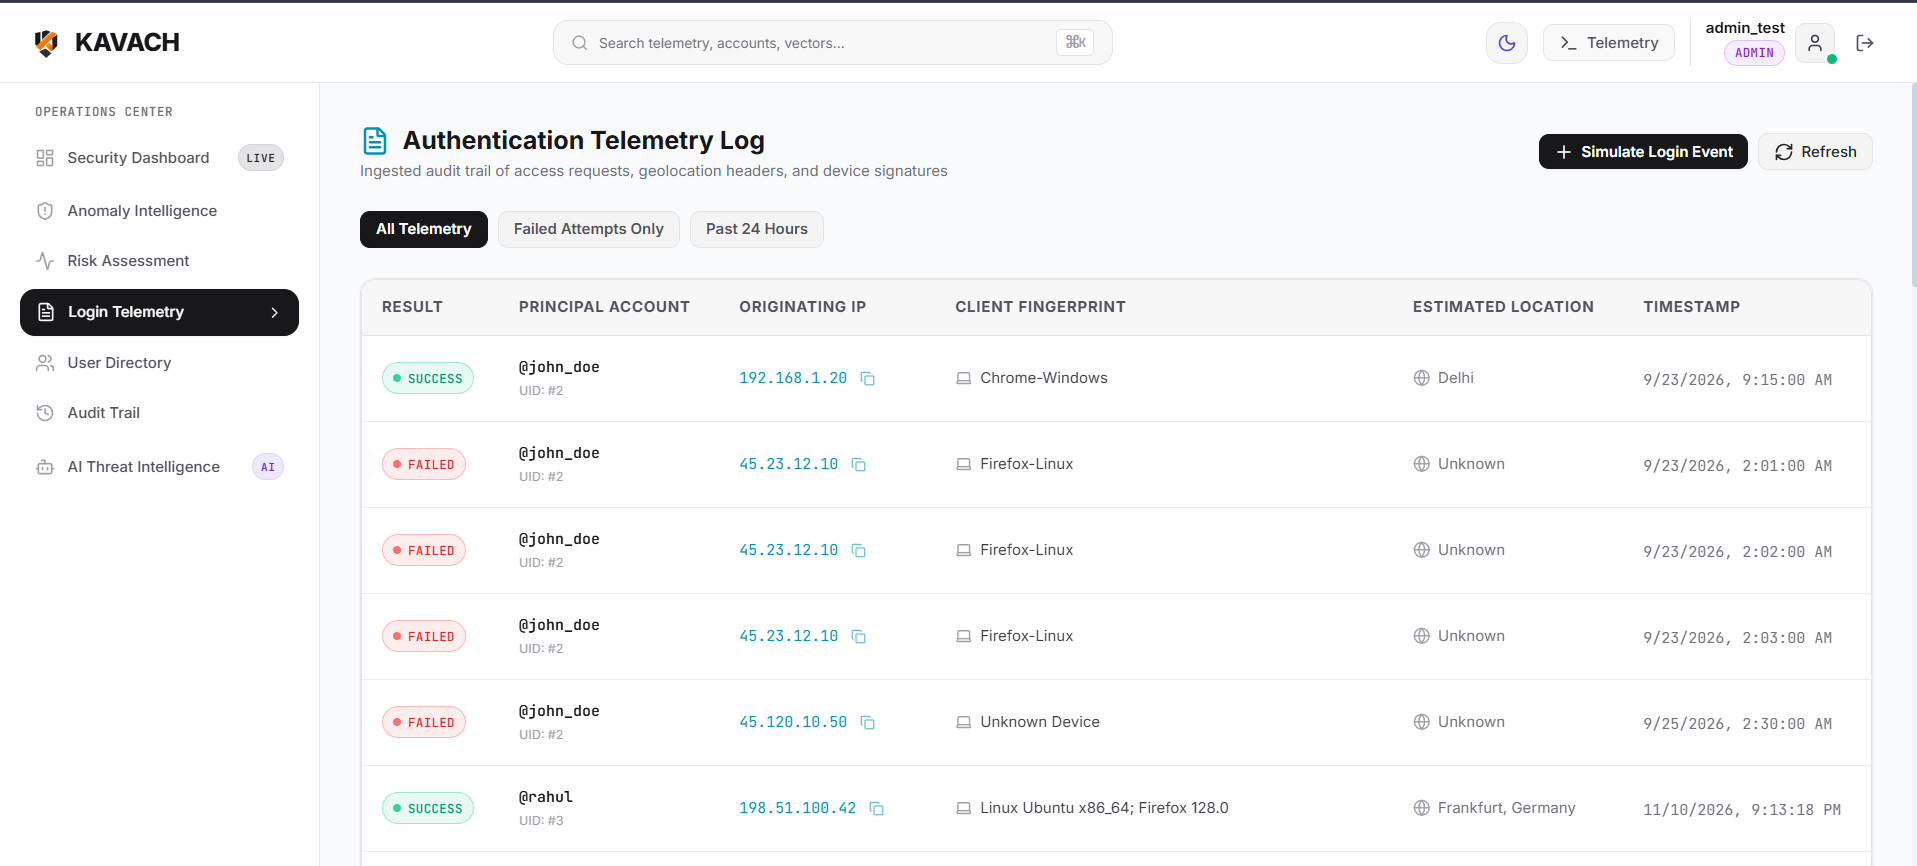
\includegraphics[width=\textwidth]{images/screenshot-telemetry.png}
\caption{Login telemetry showing successful and failed events with account and client metadata.}\label{fig:screen-telemetry}
\end{figure}

\clearpage\subsection{Personal Risk and AI Workspace}
The personal page shows the signed-in account's risk profile. Its recent 24-hour score and historical anomaly counts cover different periods. Although the interface uses subtitles such as ``Bayesian'' and ``neural'', Chapter 4 describes the implemented fixed rules and additive score. The AI screenshot captures the initial console before any completed model or tool execution.

\begin{figure}[!ht]\centering
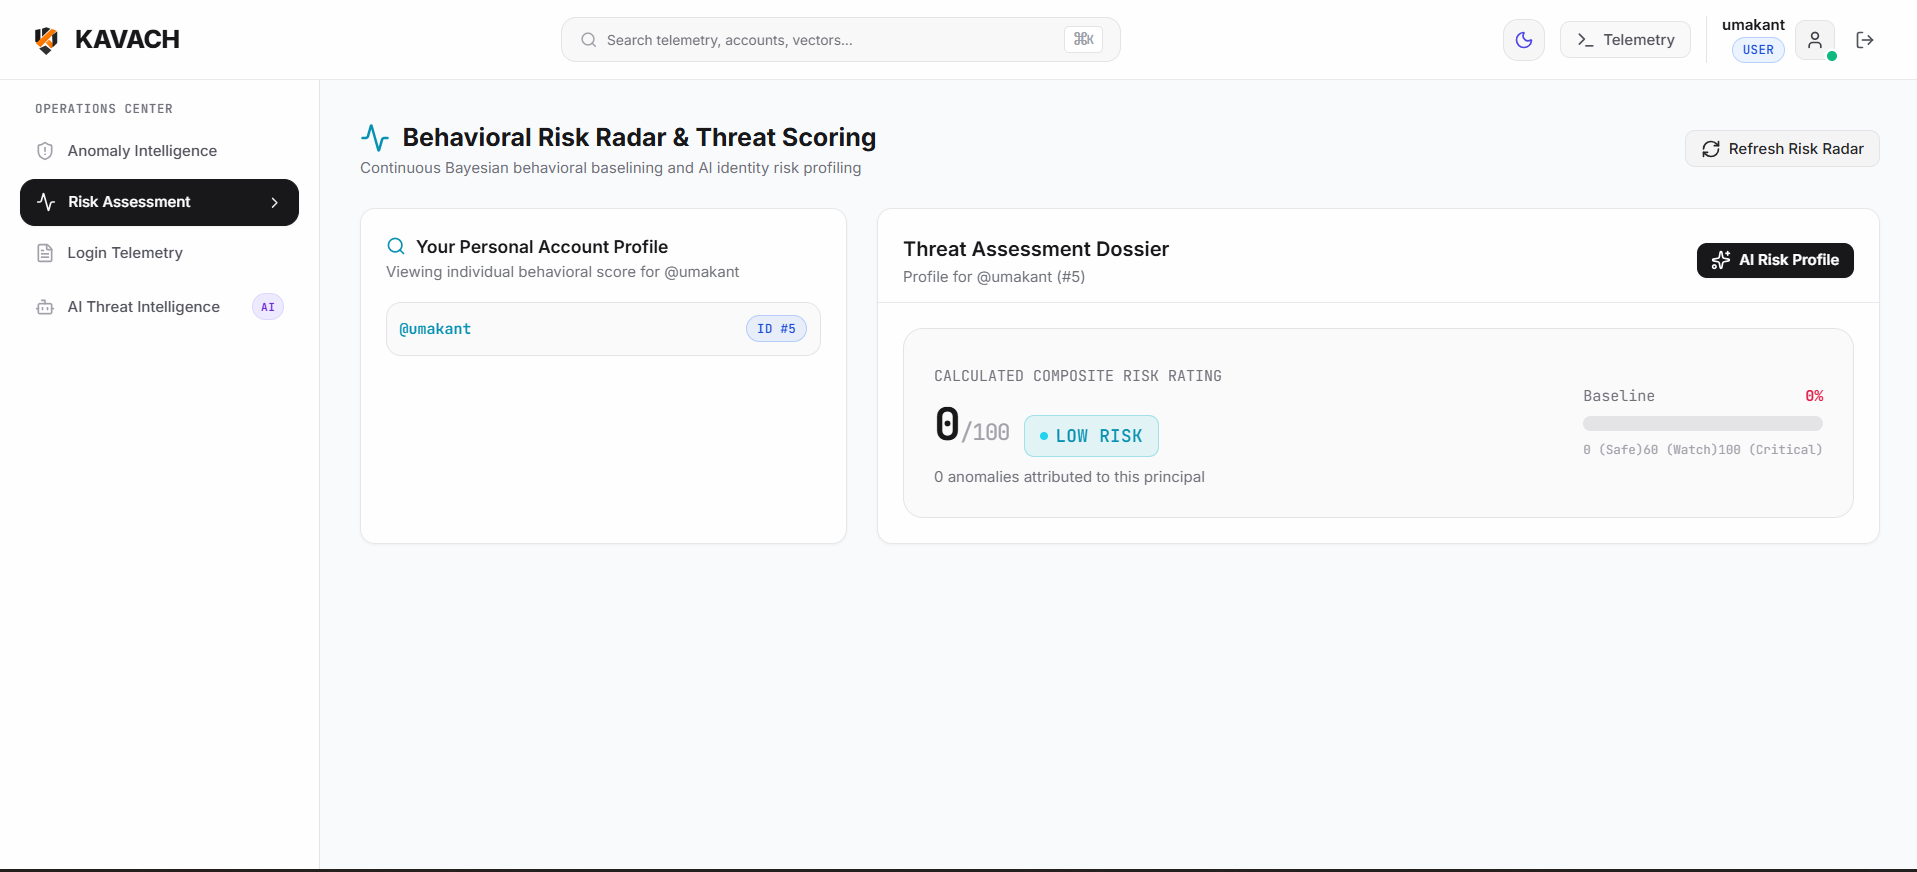
\includegraphics[width=\textwidth]{images/screenshot-personal-risk.png}
\caption{Personal risk view for the USER account, showing the displayed score and profile.}\label{fig:screen-risk}
\end{figure}

\begin{figure}[!ht]\centering
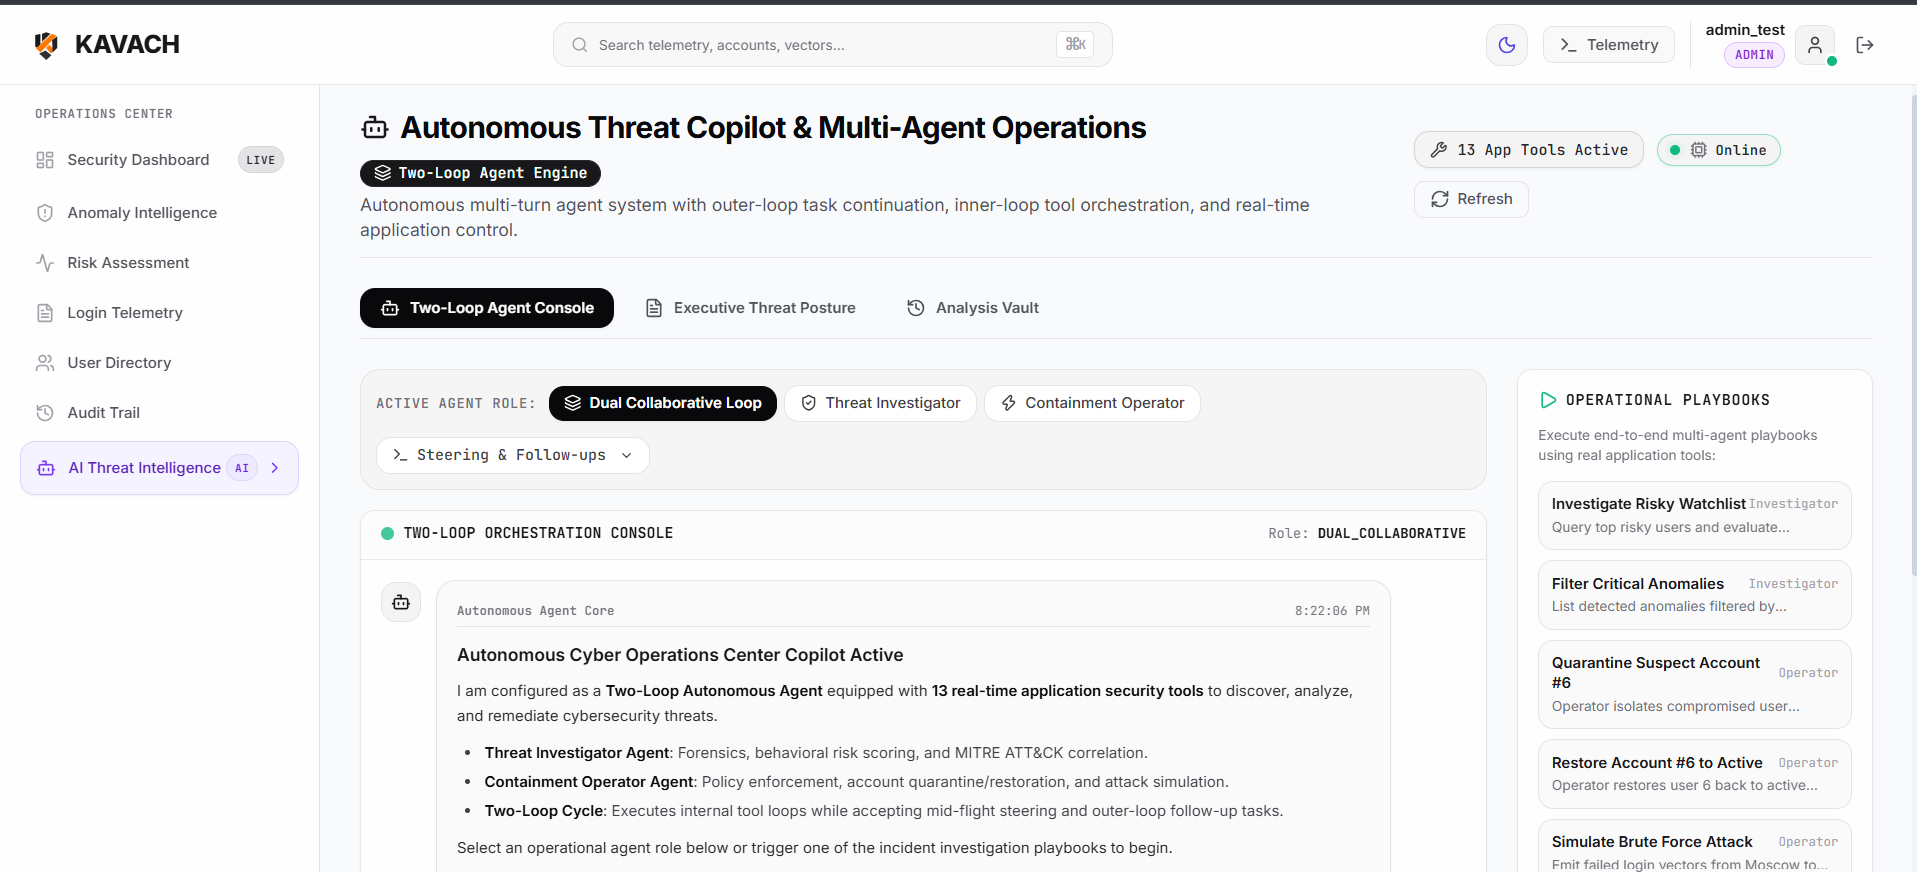
\includegraphics[width=\textwidth]{images/screenshot-ai-console.png}
\caption{AI workspace with agent-role selection, a 13-tool indicator, and operational playbooks.}\label{fig:screen-ai}
\end{figure}


\clearpage\section{Validation Plan}
The screenshots show interface states captured by the candidate. The repository has a context-loading test, but the project materials contain no controlled rule-test or load-test results. Table~\ref{tab:tests} defines the inputs and expected outcomes for validation; none of these rows records a test pass.
\begingroup\footnotesize\setstretch{1.0}\renewcommand{\arraystretch}{1.1}\setlength{\parskip}{0pt}
\begin{longtable}{>{\raggedright\arraybackslash}p{0.9cm}>{\raggedright\arraybackslash}p{6.1cm}>{\raggedright\arraybackslash}p{7cm}}
\caption{Functional validation plan; execution pending.}\label{tab:tests}\\\toprule ID & Input / action & Expected behavior to verify\\\midrule\endfirsthead
\toprule ID & Input / action & Expected behavior to verify\\\midrule\endhead
T1 & Register unique credentials. & Active USER, encoded password, safe response, audit event.\\
T2 & Repeat username or email. & Conflict and no duplicate account.\\
T3 & Valid password for active user. & JWT, success telemetry, applicable contextual rules.\\
T4 & Incorrect password for known user. & Unauthorized; failed telemetry and failed-login anomaly.\\
T5 & Unknown username. & Audit failure; no user-linked login record.\\
T6 & Inactive account attempts login. & Forbidden; failed telemetry and inactive-user anomaly.\\
T7 & Events at 04:59 and 05:00. & Unusual-time alert only before 05:00.\\
T8 & First event, repeated values, unseen IP/device. & No initial new-value alerts; later unseen values trigger.\\
T9 & Four then five failures in window. & Fifth qualifying failure adds brute-force anomaly.\\
T10 & Reanalyse identical login event. & No duplicate event/user/rule anomaly in sequential execution.\\
T11 & Weight totals 29, 30, 59, 60, 79, 80, 120. & Correct boundary tiers; score capped at 100.\\
T12 & Move anomaly detection time beyond 24 hours. & Expired anomaly excluded from risk.\\
T13 & Deactivate account with issued JWT. & Subsequent protected request rejected.\\
T14 & Make live inference unavailable. & Deterministic fallback with accurate status and outcomes.\\
T15 & Submit steering and two follow-ups. & Inner context consumes steering; outer cycles consume follow-ups.\\\bottomrule
\end{longtable}
\endgroup

Further tests must check cross-account access and administrative actions through both endpoints and tools. They must also cover invalid arguments, malformed model output, provider failures, concurrent inserts, and backdated events.

Detection evaluation requires labelled ordinary and suspicious events, with precision and recall measured for each rule. Performance results must record hardware, data volume, concurrency, latency, and whether inference was live or in fallback mode. Deterministic and model-assisted results need separate measurements.
\chapter{Conclusion and Future Work}
\section{Conclusion}
KAVACH records authenticated login activity, applies six explicit detection rules, and calculates a capped 24-hour account risk score. Security views and audit records support investigation. The LLM interface connects requests to thirteen application tools through a two-loop service, with deterministic fallback when live inference is unavailable. The repository and screenshots show the implementation and interface design. Detection accuracy and production performance still require measurement.

\noindent\textbf{Limitations.}
Fixed login hours and comparisons of IP or device strings can identify unusual values without establishing account compromise. The weights remain uncalibrated. The brute-force query has no explicit upper time bound, and duplicate prevention needs concurrency testing. Steering is local to each request, tools run sequentially, and operational tools need consistent authorization. Storing audit records alone provides no demonstrated tamper resistance.

\noindent\textbf{Future work.}
The next priorities are a centralized authorization policy for tools, reliable event-time handling, database constraints, and integration tests for each rule. Agent sessions need authentication, cancellation, and live steering. Audit retention needs protection, and query limits and concurrent performance need testing. A labelled evaluation corpus should guide threshold calibration before adding learned anomaly models, external SIEM integration, or more authentication factors.

\begin{thebibliography}{9}
\bibitem{repo} KAVACH project source, \emph{login-analysis-backend} and \emph{login-analysis-frontend}, local snapshot reviewed 17 November 2026. Project structure in Appendix A.
\bibitem{jwt} M. Jones, J. Bradley, and N. Sakimura, \emph{JSON Web Token (JWT)}, RFC 7519, May 2015. \url{https://www.rfc-editor.org/rfc/rfc7519}.
\bibitem{spring} Spring, \emph{Spring Security Reference: Method Security}. \url{https://docs.spring.io/spring-security/reference/servlet/authorization/method-security.html}. Accessed 17 November 2026.
\bibitem{owasp} OWASP Foundation, \emph{Logging Cheat Sheet}. \url{https://cheatsheetseries.owasp.org/cheatsheets/Logging_Cheat_Sheet.html}. Accessed 17 November 2026.
\bibitem{template} NIT Agartala, \emph{B.Tech 7th Semester LaTeX Template}, user-supplied archive including institutional class, logos, and chapter styling; adapted for MCA.
\end{thebibliography}
\appendix% Supporting material after References.
\chapter{Project Structure}
\section{Repository Organization}
The REST backend and browser frontend occupy separate directories. This tree lists the implementation files and folders, excluding generated builds, installed dependencies, and local configuration values.
\begingroup\footnotesize\setstretch{1.0}
\begin{lstlisting}[basicstyle=\ttfamily\scriptsize]
UserLoginProject/
  login-analysis-backend/
    pom.xml, mvnw, mvnw.cmd
    src/main/java/com/loginanalysis/
      LoginAnalysisBackendApplication.java
      config/       JWT filter, security, passwords, AI setup
      controller/   REST entry points
      dto/          Request and response contracts
      entity/       JPA model
      repository/   Queries and aggregates
      service/      Business logic
      agent/
        TwoLoopAgentService.java
        model/      Roles, messages, tools, execution steps
        tools/      SecurityToolsRegistry.java
      util/         Provider and request helpers
      exception/    Application errors
    src/main/resources/application.properties
    src/test/java/com/loginanalysis/
      LoginAnalysisBackendApplicationTests.java
  login-analysis-frontend/
    package.json, vite.config.js
    public/
    src/
      App.jsx, main.jsx
      api/          HTTP client and feature APIs
      context/      Authentication and theme
      pages/        Feature pages
      components/   Layout and reusable UI
      utils/        Logging and animation
      assets/
\end{lstlisting}
\endgroup



\chapter{Database Tables}
The tables list JPA attributes, Java types, and any explicitly declared column names. PK denotes a primary key, FK a relationship, NN non-null, and UQ unique. All identifiers are identity-generated Long values, and enums use string storage. Initialization values are application defaults without implied SQL DEFAULT clauses. ORM configuration determines physical naming.

\section{Users}
\begingroup\footnotesize\setstretch{1.0}\setlength{\parskip}{0pt}\renewcommand{\arraystretch}{1.15}
\begin{longtable}{>{\raggedright\arraybackslash}p{4.5cm}>{\raggedright\arraybackslash}p{2.2cm}>{\raggedright\arraybackslash}p{1.4cm}>{\raggedright\arraybackslash}p{5.7cm}}
\caption{Data dictionary: \code{users}.}\\\toprule Attribute & Type & Mapping & Purpose / initialization\\\midrule\endfirsthead
\toprule Attribute & Type & Mapping & Purpose / initialization\\\midrule\endhead
\code{id} & Long & PK & Identity-generated account identifier.\\
\code{username} & String & NN, UQ & Up to 100 characters.\\
\code{email} & String & NN, UQ & Up to 150 characters; normalized during registration.\\
\code{password} & String & NN & Encoded password; authentication uses BCrypt matching.\\
\code{active} & Boolean & NN & Initialized to true; false blocks account access.\\
\code{role} & UserRole & NN & String enum, length 20; initialized to USER when absent.\\
\code{createdAt} & LocalDate\allowbreak{}Time & NN & Set on creation when absent.\\\bottomrule
\end{longtable}\endgroup

A user can have many login, anomaly, and analysis-history records. Audit records store usernames without a relationship to \code{users}. UserRole has two values: ADMIN and USER.

\section{Login Events}
\begingroup\footnotesize\setstretch{1.0}\setlength{\parskip}{0pt}\renewcommand{\arraystretch}{1.15}
\begin{longtable}{>{\raggedright\arraybackslash}p{4.5cm}>{\raggedright\arraybackslash}p{2.2cm}>{\raggedright\arraybackslash}p{1.4cm}>{\raggedright\arraybackslash}p{5.7cm}}
\caption{Data dictionary: \code{user_login_logs}.}\\\toprule Attribute / column & Type & Mapping & Purpose\\\midrule\endfirsthead
\toprule Attribute / column & Type & Mapping & Purpose\\\midrule\endhead
\code{id} & Long & PK & Login-event identifier.\\
\code{user} / \code{user_id} & User & FK, NN & Required many-to-one, lazy user reference.\\
\code{loginTime} / \code{login_time} & LocalDate\allowbreak{}Time & NN & Event timestamp; initialized when absent.\\
\code{ipAddress} / \code{ip_address} & String & NN & Up to 100 characters.\\
\code{location} & String & Optional & Up to 100 characters; event-supplied context.\\
\code{device} & String & Optional & Up to 200 characters; device/user-agent string.\\
\code{status} & LoginStatus & NN & String enum, length 20: SUCCESS or FAILED.\\\bottomrule
\end{longtable}\endgroup
The declared indexes cover \code{user_id}, \code{login_time}, \code{status}, and \code{ip_address}, named \code{idx_login_username}, \code{idx_login_time}, \code{idx_login_status}, and \code{idx_login_ip}, respectively. The name \code{idx_login_username} thus refers to an index on the user identifier.

\section{Anomalies}
\begingroup\footnotesize\setstretch{1.0}\setlength{\parskip}{0pt}\renewcommand{\arraystretch}{1.15}
\begin{longtable}{>{\raggedright\arraybackslash}p{4.5cm}>{\raggedright\arraybackslash}p{2.2cm}>{\raggedright\arraybackslash}p{1.4cm}>{\raggedright\arraybackslash}p{5.7cm}}
\caption{Data dictionary: \code{anomalies}.}\\\toprule Attribute / column & Type & Mapping & Purpose\\\midrule\endfirsthead
\toprule Attribute / column & Type & Mapping & Purpose\\\midrule\endhead
\code{id} & Long & PK & Anomaly identifier.\\
\code{user} / \code{user_id} & User & FK, NN & Required many-to-one account reference.\\
\code{loginLog} / \code{login_log_id} & LoginLog & FK, NN & Required triggering-event reference.\\
\code{anomalyType} & AnomalyType & NN & One of the six rule types.\\
\code{description} & String & NN & Human-readable trigger explanation.\\
\code{riskScore} & Integer & NN & Fixed weight assigned by the matching rule.\\
\code{severity} & Severity & NN & LOW, MEDIUM, HIGH, or CRITICAL.\\
\code{detectedAt} & LocalDate\allowbreak{}Time & NN & Detection timestamp initialized when saved.\\\bottomrule
\end{longtable}\endgroup

AnomalyType has six values: \code{FAILED_LOGIN}, \code{UNUSUAL_LOGIN_TIME}, \code{INACTIVE_USER_LOGIN}, \code{NEW_IP}, \code{NEW_DEVICE}, and \code{BRUTE_FORCE}. The service searches for the same user/type/login combination before saving. The entity has no composite uniqueness constraint for that combination.

\section{AI Analysis History}
\begingroup\footnotesize\setstretch{1.0}\setlength{\parskip}{0pt}\renewcommand{\arraystretch}{1.15}
\begin{longtable}{>{\raggedright\arraybackslash}p{4.5cm}>{\raggedright\arraybackslash}p{2.2cm}>{\raggedright\arraybackslash}p{1.4cm}>{\raggedright\arraybackslash}p{5.7cm}}
\caption{Data dictionary: \code{ai_analysis_history}.}\\\toprule Attribute / column & Type & Mapping & Purpose\\\midrule\endfirsthead
\toprule Attribute / column & Type & Mapping & Purpose\\\midrule\endhead
\code{id} & Long & PK & Analysis record identifier.\\
\code{anomaly} / \code{anomaly_id} & Anomaly & FK, optional & Lazy link to the analyzed anomaly.\\
\code{user} / \code{user_id} & User & FK, optional & Lazy link to the associated user.\\
\code{cachedAnomalyId} & Long & Optional & Column \code{cached_anomaly_id}; retained identifier, not FK.\\
\code{cachedUserId} & Long & Optional & Column \code{cached_user_id}; retained identifier, not FK.\\
\code{username} & String & Optional & Up to 100 characters.\\
\code{analysisType} & String & NN & Up to 50 characters.\\
\code{summary} & String / TEXT & Optional & Generated or fallback overview.\\
\code{riskExplanation} & String / TEXT & Optional & Contextual risk explanation.\\
\code{indicatorsJson} & String / TEXT & Optional & Serialized indicators.\\
\code{recommendationsJson} & String / TEXT & Optional & Serialized recommendations.\\
\code{confidence} & String & Optional & Up to 20 characters; advisory label.\\
\code{threatLevel} & String & Optional & Up to 20 characters.\\
\code{model} & String & Optional & Up to 100 characters.\\
\code{isAdvisory} & Boolean & NN & Initialized to true.\\
\code{createdAt} & LocalDate\allowbreak{}Time & NN & Analysis creation timestamp.\\\bottomrule
\end{longtable}\endgroup

Fields labelled JSON store serialized text in TEXT columns; the entity definitions do not map them to PostgreSQL JSONB. Optional relationships and cached IDs preserve analysis context. The history service and DTO control which fields reach the caller.

\section{Audit Records}
\begingroup\footnotesize\setstretch{1.0}\setlength{\parskip}{0pt}\renewcommand{\arraystretch}{1.15}
\begin{longtable}{>{\raggedright\arraybackslash}p{4.5cm}>{\raggedright\arraybackslash}p{2.2cm}>{\raggedright\arraybackslash}p{1.4cm}>{\raggedright\arraybackslash}p{5.7cm}}
\caption{Data dictionary: \code{audit_logs}.}\\\toprule Attribute & Type & Mapping & Purpose\\\midrule\endfirsthead
\toprule Attribute & Type & Mapping & Purpose\\\midrule\endhead
\code{id} & Long & PK & Audit record identifier.\\
\code{username} & String & Optional & Actor/account text; no declared user FK.\\
\code{action} & String & NN & Security or application action name.\\
\code{details} & String & Optional & Description, up to 1000 characters.\\
\code{ipAddress} & String & Optional & Recorded request/action source.\\
\code{timestamp} & LocalDate\allowbreak{}Time & NN & Initialized when absent.\\\bottomrule
\end{longtable}\endgroup
This table stores selected audit events. Its entity mapping provides no append-only restriction, hash chain, or database trigger that records every change.

\chapter{API Quick Reference}
Every route has the prefix \code{/api}; \code{:name} marks a path variable. Public routes need no token. ADMIN and USER are application roles. Owner permits an administrator or the verified account owner, while Signed-in requires general authentication. These scopes follow source declarations and have not been verified by executed authorization tests. Agent tools need a separate execution policy.

\section{Authentication and Directory}
\begingroup\footnotesize\setstretch{1.0}\setlength{\parskip}{0pt}\renewcommand{\arraystretch}{1.15}
\begin{longtable}{>{\raggedright\arraybackslash}p{1.5cm}>{\raggedright\arraybackslash}p{5.9cm}>{\raggedright\arraybackslash}p{1.8cm}>{\raggedright\arraybackslash}p{4.6cm}}
\caption{Authentication and user-directory endpoints.}\\\toprule Method & Route after /api & Scope & Purpose\\\midrule\endfirsthead
\toprule Method & Route after /api & Scope & Purpose\\\midrule\endhead
POST & \code{/auth/register} & Public & Register an active USER; returns 201 and safe account details.\\
POST & \code{/auth/login} & Public & Verify credentials; return JWT and safe account details.\\
GET & \code{/users} & ADMIN & List accounts.\\
POST & \code{/users} & ADMIN & Create an account; returns 201.\\
GET & \code{/users/:id} & ADMIN & Retrieve an account.\\
PUT & \code{/users/:id} & ADMIN & Update account using UserRequestDTO.\\
PATCH & \code{/users/:id/status?active=false} & ADMIN & Set active state; query parameter can be true or false.\\
DELETE & \code{/users/:id} & ADMIN & Delete account; returns 204 on completion.\\\bottomrule
\end{longtable}\endgroup

Registration accepts \code{username}, \code{email}, and \code{password}. DTO limits are 3--100 characters for username, 150 for email, and 8--72 for password. Login requires a nonblank username and password with limits of 100/72 characters. A failed login for a known account attempts telemetry recording. An unknown account produces an audit failure without a user-linked login record.

\section{Telemetry and Anomalies}
\begingroup\footnotesize\setstretch{1.0}\setlength{\parskip}{0pt}\renewcommand{\arraystretch}{1.15}
\begin{longtable}{>{\raggedright\arraybackslash}p{1.5cm}>{\raggedright\arraybackslash}p{5.9cm}>{\raggedright\arraybackslash}p{1.8cm}>{\raggedright\arraybackslash}p{4.6cm}}
\caption{Login-event and anomaly endpoints.}\\\toprule Method & Route after /api & Scope & Purpose\\\midrule\endfirsthead
\toprule Method & Route after /api & Scope & Purpose\\\midrule\endhead
POST & \code{/login-logs} & ADMIN & Persist an explicit event and invoke detection.\\
GET & \code{/login-logs} & ADMIN & List login records.\\
GET & \code{/login-logs/user/:userId} & Owner & Retrieve account-specific logs.\\
GET & \code{/login-logs/failed} & ADMIN & Retrieve failed events.\\
GET & \code{/login-logs/recent?hours=24} & ADMIN & Retrieve recent events; hours defaults to 24.\\
GET & \code{/anomalies} & ADMIN & Paginated list with severity/type filters and sorting.\\
GET & \code{/anomalies/:id} & Owner & Retrieve one anomaly; check its owning account.\\
GET & \code{/anomalies/user/:userId} & Owner & List an account's anomalies.\\
GET & \code{/anomalies/user/:userId/paginated} & Owner & Paginated account anomalies and filters.\\
GET & \code{/anomalies/severity/:severity} & ADMIN & List anomalies by severity.\\
GET & \code{/anomalies/type/:type} & ADMIN & List anomalies by rule type.\\\bottomrule
\end{longtable}\endgroup

Event creation requires \code{userId}, \code{ipAddress}, and \code{status}, with optional \code{loginTime}, \code{location}, and \code{device}. Anomaly queries default to \code{page=0}, \code{size=10}, \code{sortBy=detectedAt}, and \code{direction=desc}. Page must be nonnegative and size must be 1--100. Sorting accepts \code{id}, \code{detectedAt}, \code{riskScore}, \code{severity}, and \code{anomalyType}.

\section{Risk, Dashboard, and Audit}
\begingroup\footnotesize\setstretch{1.0}\setlength{\parskip}{0pt}\renewcommand{\arraystretch}{1.15}
\begin{longtable}{>{\raggedright\arraybackslash}p{1.5cm}>{\raggedright\arraybackslash}p{5.9cm}>{\raggedright\arraybackslash}p{1.8cm}>{\raggedright\arraybackslash}p{4.6cm}}
\caption{Risk, analytics, dashboard, and audit endpoints.}\\\toprule Method & Route after /api & Scope & Purpose\\\midrule\endfirsthead
\toprule Method & Route after /api & Scope & Purpose\\\midrule\endhead
GET & \code{/risk/user/:userId} & Owner & Account's 24-hour capped risk score and tier.\\
GET & \code{/risk/dashboard} & ADMIN & Overall risk/severity summary.\\
GET & \code{/dashboard/security} & ADMIN & Combined security dashboard.\\
GET & \code{/dashboard/top-risky-users} & ADMIN & Ranked watchlist, up to ten accounts.\\
GET & \code{/dashboard/recent-critical-anomalies} & ADMIN & Recent critical anomalies.\\
GET & \code{/analytics/logins} & Signed-in & Login counts, failure rate, seven-day trend.\\
GET & \code{/audit-logs} & ADMIN & All persisted audit records.\\
GET & \code{/audit-logs/user/:username} & ADMIN & Audit records for a username.\\
GET & \code{/audit-logs/action/:action} & ADMIN & Audit records for an action.\\\bottomrule
\end{longtable}\endgroup

Login analytics inherits the security chain's authentication requirement and has no ADMIN-only controller annotation. The dashboard routes separately require ADMIN access.

\section{AI Analysis and Agent Execution}
\begingroup\footnotesize\setstretch{1.0}\setlength{\parskip}{0pt}\renewcommand{\arraystretch}{1.15}
\begin{longtable}{>{\raggedright\arraybackslash}p{1.5cm}>{\raggedright\arraybackslash}p{5.9cm}>{\raggedright\arraybackslash}p{1.8cm}>{\raggedright\arraybackslash}p{4.6cm}}
\caption{AI and two-loop agent endpoints.}\\\toprule Method & Route after /api & Scope & Purpose\\\midrule\endfirsthead
\toprule Method & Route after /api & Scope & Purpose\\\midrule\endhead
GET & \code{/ai/status} & ADMIN / USER & Model readiness and mode information.\\
POST & \code{/ai/analyze/anomaly/:anomalyId} & Owner & Dedicated anomaly explanation; alias below.\\
POST & \code{/ai/analyze-anomaly/:anomalyId} & Owner & Alias for anomaly explanation.\\
GET / POST & \code{/ai/analyze/security-summary} & ADMIN & Global security summary; also \code{/ai/summary}.\\
GET & \code{/ai/history} & ADMIN / USER & Paginated history; service scopes ordinary users to their own records.\\
GET & \code{/ai/history/:id} & ADMIN / USER & One history record; service checks cached owner where present.\\
POST & \code{/ai/analyze-user/:userId} & Owner & Dedicated user-risk analysis.\\
POST & \code{/ai/agent-loop} & ADMIN / USER & Execute prompt and queued steering/follow-ups; return trace.\\
GET & \code{/ai/agent-tools} & ADMIN / USER & List registered tools, schemas, roles, and safety metadata.\\
POST & \code{/ai/chat} & ADMIN / USER & Run agent from prompt/context; return simplified chat response.\\\bottomrule
\end{longtable}\endgroup


Agent execution requires a nonblank prompt. One request can also supply context, a role, steering messages, and follow-up arrays. The roles are investigator, operator, and collaborative. Responses contain final text, execution steps, tool names, loop counts, model/mode, and completion time.

Reads and analysis normally return 200. Declared creation routes return 201, and deletion returns 204. Errors use 400 for invalid input, 401 for credentials or tokens, 403 for denied access, 404 for a missing resource, and 409 for duplicate registration. Operational tools can change data in both fallback and live inference modes.

\chapter{Publications Related to the Work}
No publications related to this project have been reported.

\chapter{Biographical Sketch}
\begin{center}
{\large\bfseries\CandidateName}\par
\vspace{0.3cm}
Department of Computer Science and Engineering\\
National Institute of Technology, Agartala, Tripura, India\\
E-mail: \href{mailto:ukbhai24@gmail.com}{ukbhai24@gmail.com}\\
Contact No.: 8789817421
\end{center}
\vspace{0.2cm}
\begingroup\renewcommand{\labelitemi}{\(\bullet\)}
\begin{itemize}
\setlength{\itemsep}{5pt}
\setlength{\parskip}{0pt}
\item \textbf{Postgraduate degree.} Master of Computer Applications (2024--2027), NIT Agartala. CGPA: 8.47/10 (ongoing).
\item \textbf{Undergraduate degree.} Bachelor of Science (Mathematics), Ranchi University. CGPA: 8.23.
\item \textbf{Intermediate education.} Physics, Chemistry and Mathematics (PCM), Jharkhand Academic Council Board, with 77.80\%.
\item \textbf{Secondary education (Class X).} S. B. N. High School, Banka Bhandar, with 84.40\%.
\item \textbf{Projects.} Developer of KAVACH: User Login Analysis Using LLM.
\end{itemize}
\endgroup


\end{document}
